\documentclass[11pt,oneside]{book}
\usepackage{ctex}
\usepackage{amsmath}
\usepackage{amsfonts}
\usepackage{graphicx}
\usepackage{animate}
\usepackage{subfigure}
\usepackage{float}
%%%%%%%%%%%%% Geometry
\usepackage[a4paper,left=2.5cm,right=2.5cm, bottom=2.5cm,top=2.5cm]{geometry}

%%%%%%%%%%%%%%% Les paquets

\usepackage[english]{babel}
\usepackage[palette=munch]{nexus}
%\usepackage{graphicx}

%%%%%%%%%%%%%%%% hyperref
\usepackage{lipsum}
\usepackage[verbose]{hyperref}
\hypersetup{ 
    hidelinks
}
\setlength{\XeTeXLinkMargin}{-1pt}


\begin{document}

\pagestyle{empty}

\definecolor{plop}{HTML}{4D7186}
\begin{textblock}{1}(0,0)
    \noindent\textcolor{plop}{\rule{\paperwidth}{.55\paperheight}}
\end{textblock}


\begin{textblock}{1}(0,.55)
    \noindent\textcolor{black}{\rule{\paperwidth}{.45\paperheight}}
\end{textblock}


\begin{textblock}{1}(.1,.09)
    \noindent{\fontsize{24.88}{2}\selectfont
        \bfseries\textcolor{white}{学习笔记}}
\end{textblock}

\begin{textblock}{1}(.1,.15)
    \noindent {\fontsize{24.88}{2}\selectfont
    \bfseries\textcolor{white}{深度学习:从MLP到GNN}}
\end{textblock}

% \begin{textblock}{1}(.1,.21)
%     \noindent{\fontsize{30}{2}\selectfont
%         \bfseries\textcolor{white}{for \LaTeX}}
% \end{textblock}

\begin{textblock}{1}(.1,.45)
    \noindent {\fontsize{20.74}{2}\selectfont
        \bfseries\textcolor{white}{李开运}}
\end{textblock}



\begin{textblock}{.9}(.05,.56)
    \begin{flushright}
        \noindent {\fontsize{20.74}{2}\selectfont
            \bfseries\textcolor{orange}{version 1.1}}
    \end{flushright}
\end{textblock}


\begin{textblock}{.45}(.5,.82)
    \begin{center}
        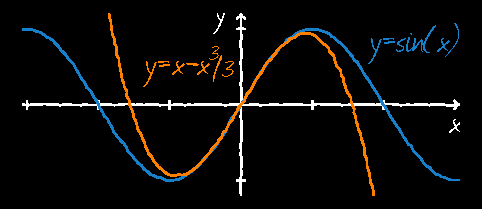
\includegraphics[width=.45\paperwidth]{./chapter/cover/dlsin}
    \end{center}
\end{textblock}

\begin{textblock}{.4}(.05,.65)
    \begin{center}
        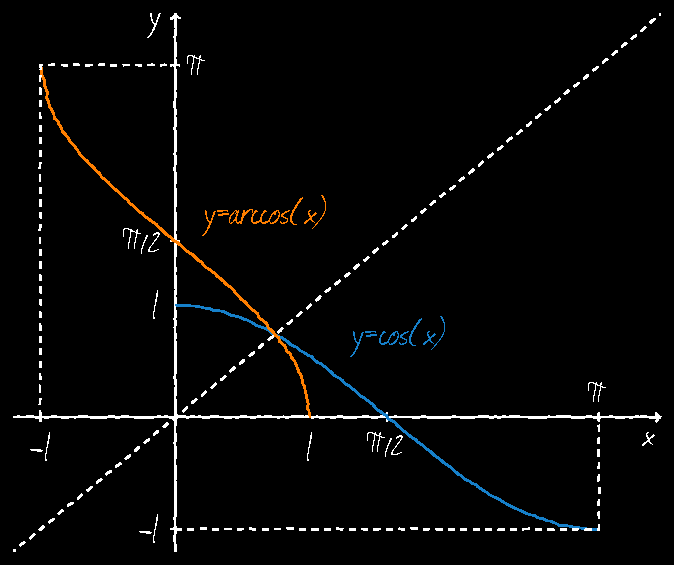
\includegraphics[width=.4\paperwidth]{./chapter/cover/arccos}
    \end{center}
\end{textblock}


\begin{textblock}{.6}(.05,.6)
    \noindent {\fontsize{20.74}{18}%
    \textcolor{white}{$\displaystyle(a+b)^n = \sum_{k=0}^n 
                \binom{n}{k} a^kb^{n-k}$}}
\end{textblock}


\begin{textblock}{.4}(.4,.77)
    \noindent {\fontsize{17.28}{18}%
    \textcolor{white!80}{$\displaystyle 
                \neg (p\vee q) \equiv (\neg p)\wedge (\neg q)$}}
\end{textblock}

\begin{textblock}{.4}(.1,.93)
    \noindent {\fontsize{14.4}{18}%
    \textcolor{white!50}{$\displaystyle 
                \binom{n}{k} = \frac{n!}{k!(n-k)!}$}}
\end{textblock}


\begin{textblock}{.6}(.5,.69)
    \noindent {\fontsize{17.28}{18}%
    \textcolor{white!10}{$\displaystyle 
                \zeta_k = |a|^{1/n} \mathrm{e}^{i(\mathrm{arg}(a)+2k\pi)/n}$}}
\end{textblock}


\begin{textblock}{.3}(.75,.73)
    \noindent {\fontsize{17.28}{18}%
    \textcolor{white!10}{$\displaystyle \mathrm{e}^{i\pi}+1=0$}}
\end{textblock}



\null\newpage\pagestyle{nexus}

\tableofcontents
\chapter{基本概念}
\chapter{深度学习基础}
\chapter{多层感知机}
test
\section{反向传播}
前向传递输入信号直至产生误差,反向传播误差信息更新权重矩阵。误差反向传播的目标是寻找一计算前馈神经网络的误差函数$E(\boldsymbol{w})$的梯度的一种高效的方法。

许多实际应用中使用的误差函数,例如针对一组独立同分布的数据的最大似然方法定义的误差函数,由若干的求和式组成,每一项对应于训练集的一个数据点,即
\begin{equation}
E(\boldsymbol{w})=\sum_{n=1}^{N}E_n(\boldsymbol{w})
\end{equation}
这里,我们要考虑的是计算$\nabla E_n(\boldsymbol{w})$的问题。这可以使用顺序优化的方法计算,或者使用批处理方法在训练集上进行累加。

首先考虑一个简单的线性模型,其中输出$y_k$是输入变量$x_i$的线性组合,即,
\begin{equation}
y_k=\sum_i w_{ki}x_i
\end{equation}
对于一个特定的输入模式n,误差函数的形式为
\begin{equation}
E_n=\frac{1}{2}\sum_k(y_{nk}-t_{nk})^2
\end{equation}
其中$y_{nk}=y_k(\boldsymbol{x}_n,\boldsymbol{w})$。这个误差函数关于一个权值$w_{ji}$的梯度为
\begin{equation}
\frac{\partial E_n}{\partial w_{ji}}=(y_{nj}-t_{nj})x_{ni}
\end{equation}
它可以表示为链接$w_{ji}$的输出端相关联的“误差信号”$y_{nj}-t_{nj}$和与链接的输入端相关联的变量$x_{nj}$的乘积。
反向传播算法可以总结如下 
\begin{enumerate}
	\item 对于网络的一个输入向量$\boldsymbol{x}_n$,使用下列进行正向传播,找到所有隐含单元和输出单元的激活。
	\begin{flalign}
	a_j&=\sum_iw_{ji}z_i\\
	z_j&=h(a_j)
	\end{flalign}
	其中$z_i$是一个单元的激活,或者是输入。它向单元j发送一个链接,$w_{ji}$是与这个链接关联的权值。
	\item 计算所有输出单元的$\delta_k$
	\begin{equation}
	\delta_k=y_k-t_k
	\end{equation}
	\item 获得网络中所有隐含单元的$\delta_j$
	\begin{equation}
	\begin{aligned}
	\delta_j\equiv \frac{\partial E_n}{\partial a_j}&=\sum_k \frac{\partial E_n}{\partial a_k}\frac{\partial a_k}{\partial a_j}\\
	&=h^{'}(a_j)\sum_k w_{kj}\delta_k
	\end{aligned}
	\end{equation}
	其中求和式的作用对象是所有向单元j发送链接的单元k。注意,单元k可以包含其他的隐含单元和输出单元。
	\item 计算导数
	\begin{equation}
	\frac{\partial E_n}{\partial w_{ji}}=\delta_jz_i
	\end{equation}
\end{enumerate}
对于批处理方法,总误差函数E的导数可以通过下面的方式得到:对于训练集里的每个模式,重复上面的步骤,然后对所有的模式求和,即
\begin{equation}
\frac{\partial E}{\partial w_{ji}}=\sum_{n}\frac{\partial E_n}{\partial w_{ji}}
\end{equation}
上面的推导中,我们隐式地假设网络中的每个隐含单元或输入单元相同的激活函数$h(\cdot)$。
\chapter{激活函数}

激活函数的作用是为模型引入非线性,提高模型的表达能力。
\begin{figure}[H]
	\centering
	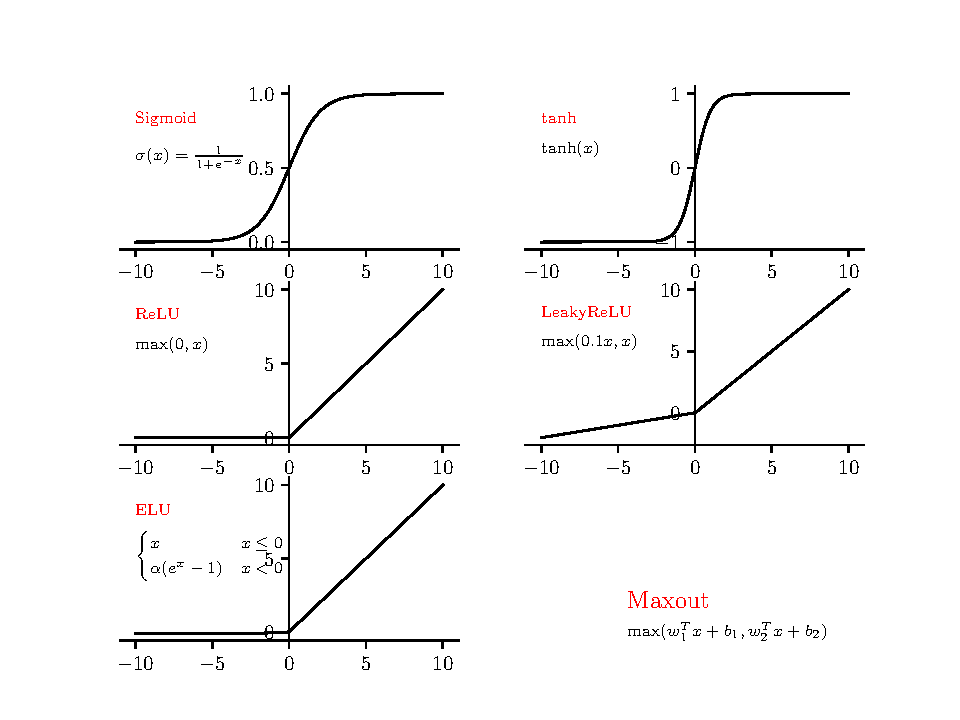
\includegraphics{./img/code/DP/activation.pdf}
\end{figure}

\chapter{损失函数}
\chapter{优化算法}
梯度下降是目前神经网络使用最为广泛的优化算法之一。可以用下述步骤描述梯度下降的流程:
\begin{enumerate}
	\item 计算目标函数关于参数的梯度
	\begin{equation}
		\boldsymbol{g}_t = \nabla_{\theta} J(\theta)
	\end{equation}
	\item 根据历史梯度计算一阶和二阶动量
	\begin{equation}
		\begin{aligned}
			\boldsymbol{m}_t &= \phi(\boldsymbol{g}_1, \boldsymbol{g}_2, \dots, \boldsymbol{g}_t) \\
			\boldsymbol{v}_t &= \psi(\boldsymbol{g}_1, \boldsymbol{g}_2, \dots, \boldsymbol{g}_t)
		\end{aligned}
	\end{equation}
	\item 更新模型参数
	\begin{equation}
		\theta_{t+1} = \theta_{t} - \frac{1}{\sqrt{v_t + \epsilon}}\boldsymbol{m}_t
	\end{equation}
\end{enumerate}

其中,$\epsilon$为平滑项,防止分母为零,通常取1e-8。
\section{小批量随机梯度下降}
小批量随机梯度下降在每次迭代中随机均匀采样多个样本来组成一个小批量,然后使用这个小批量来计算梯度。没有动量的概念,即$\boldsymbol{m}_t=\eta \boldsymbol{g}_t, \boldsymbol{v}_t=I^2,\epsilon = 0$
\begin{equation}
\begin{aligned}
	\boldsymbol{g}_t \leftarrow \nabla J_{\mathcal{B}_t}(\boldsymbol{x}_{t-1})  &= \frac{1}{|\mathcal{B}|}\sum_{i \in \mathcal{B}_t}\nabla J_i(\boldsymbol{x}_{t-1})\\
	\theta_{t+1} &= \theta_{t} - \eta \boldsymbol{g}_t
\end{aligned}
\end{equation}
SGD的缺点在于收敛速度慢,可能在鞍点处震荡。并且,如何合理的选择学习率是SGD的一大难点。
\section{动量法}
SGD在遇到沟壑时容易陷入震荡。为此,可以为其引入动量Momentum,加速SGD在正确方向的下降并抑制震荡。
\begin{equation}
\begin{aligned}
	\boldsymbol{m}_t&=\gamma \boldsymbol{m}_{t-1} + \eta \boldsymbol{g}_t\\
	\theta_{t+1} &= \theta_{t} - \boldsymbol{m}_t
\end{aligned}
\end{equation}
这意味着参数更新方向不仅由当前的梯度决定,也与此前累积的下降方向有关。这使得参数中那些梯度方向变化不大的维度可以更新,并减少梯度方向变较大的维度上的更新幅度。由此产生了加速收敛和减小震荡的效果。

动量法使用了指数加权移动平均的思想。它将过去时间步的梯度做了加权平均,且权重按时间步指数衰减。动量法使得相邻时间步的自变量更新在方向上更加一致。
\section{AdaGrad算法}
深度学习模型中往往涉及大量的参数,不同参数的更新频率往往有所区别。对于更新不频繁的参数,我们希望单次步长更大,多学习一些知识;对于更新频率的参数,我们则希望步长较小,使得学习到的参数更稳定,不至于被单个样本影响太多。

Adagrad算法引入了二阶动量:
\begin{equation}
	\begin{aligned}
		\boldsymbol{v}_t&=\mathrm{diag}(\sum_{i=1}^{t}\boldsymbol{g}_{i,1}^2, \sum_{i=1}^{t}\boldsymbol{g}_{i,2}^2, \dots, \sum_{i=1}^{t}\boldsymbol{g}_{i,d}^2)\\
		\theta_{t+1} &= \theta_{t} - \frac{\eta}{\sqrt{v_t + \epsilon}}\boldsymbol{g}_t
	\end{aligned}
\end{equation}
AdaGrad算法在迭代过程中不断调整学习率,并让目标函数自变量中每个元素都分别拥有自己的学习率。使用AdaGrad算法时,自变量中每个元素的学习率在迭代过程中一直在降低(或不变)。这一方法在稀疏数据的场景下表现很好。
\section{RMSProp算法}
在Adagrad中,$v_t$是单增的,使得学习率逐渐递减至0,可能导致训练过程提前结束。为了改进这一缺点,可以考虑在计算二阶动量时不累积全部历史梯度,而只关注最近某一时间窗口内的下降梯度。根据此思想有了RMSprop。有
\begin{equation}
	\begin{aligned}
		v_t &= \gamma v_{t-1} + (1-\gamma)\cdot \mathrm{diag}(g_t \odot g_t)\\
		\theta_{t+1} &= \theta_{t} - \frac{\eta}{\sqrt{v_t + \epsilon}}\boldsymbol{g}_t
	\end{aligned}
\end{equation}
其二阶动量采用指数移动平均公式计算,这样可避免二阶动量持续累积的问题。
\section{Adam算法}
Adam可以认为是RMSprop和Momentum的结合。和RMSprop对二阶动量使用指数移动平均类似,Adam中对一阶动量也是用指数移动平均计算。
\begin{equation}
	\begin{aligned}
		\boldsymbol{m}_t&=\eta [\beta_1 \boldsymbol{m}_{t-1} + (1-\beta_1)  \boldsymbol{g}_t]\\
		\boldsymbol{v}_t &= \beta_2 \boldsymbol{v}_{t-1} + (1-\beta_2)\cdot \mathrm{diag}(\boldsymbol{g}_t \odot \boldsymbol{g}_t) 
	\end{aligned}
\end{equation}
其中,初值$\boldsymbol{m}_0=0,\boldsymbol{v}_0=0$。注意到,在迭代初始阶段,$\boldsymbol{m}_t,\boldsymbol{v}_t$有一个向初值的偏移(过多地偏向0)。因此,可以做偏置校正
\begin{equation}
\begin{aligned}
	\hat{\boldsymbol{m}}_t&=\frac{\boldsymbol{m}_t}{1-\beta_1^t}\\
	\hat{\boldsymbol{v}}_t &=  \frac{\boldsymbol{v}_t}{1-\beta_2^t}
\end{aligned}
\end{equation}
再更新
\begin{equation}
	\theta_{t+1} = \theta_{t} - \frac{1}{\sqrt{\hat{\boldsymbol{v}}_t + \epsilon}}\hat{\boldsymbol{m}}_t
\end{equation}
\section{过拟合}
\section{神经网络的扩展}
\begin{enumerate}
	\item 增加额外的处理层
	\item 引入跨层链接
	\item 稀疏网络
\end{enumerate}


\chapter{卷积神经网络}
\section{CNN}
\subsection{卷积}
信号处理中,卷积被定义为:一个函数经过翻转和移动后与另一个函数的乘积的积分.
\begin{equation}
	(f*g)(t)=\int_{-\infty}^{\infty} f(\tau)g(t-tau)\mathrm{d}\tau 
\end{equation}
在深度学习中的卷积本质上是信号处理中的互相关(cross-correlation)操作。执行卷积的目的是从输入中提取有用的特征。卷积神经网络通过卷积在训练期间使用自动学习权重的函数来提取特征,所有这些提取出来的特征之后会被组合在一起做出决策。

\begin{enumerate}
	\item 2D卷积,如图\ref{2d_conv}
	\begin{figure}[H]
		\centering
		\label{2d_conv}
		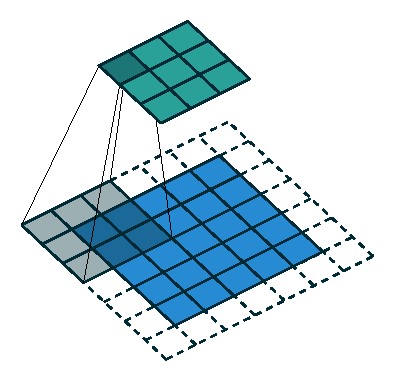
\includegraphics[width=0.3\linewidth]{./img/code/CNN/1.pdf}
		\caption{2D卷积}
	\end{figure}
	\item 多通道卷积(空间卷积),如图\ref{space_conv}
	\begin{figure}[H]
		\label{space_conv}
		\subfigure{
			\begin{minipage}[t]{\linewidth}
				\centering
				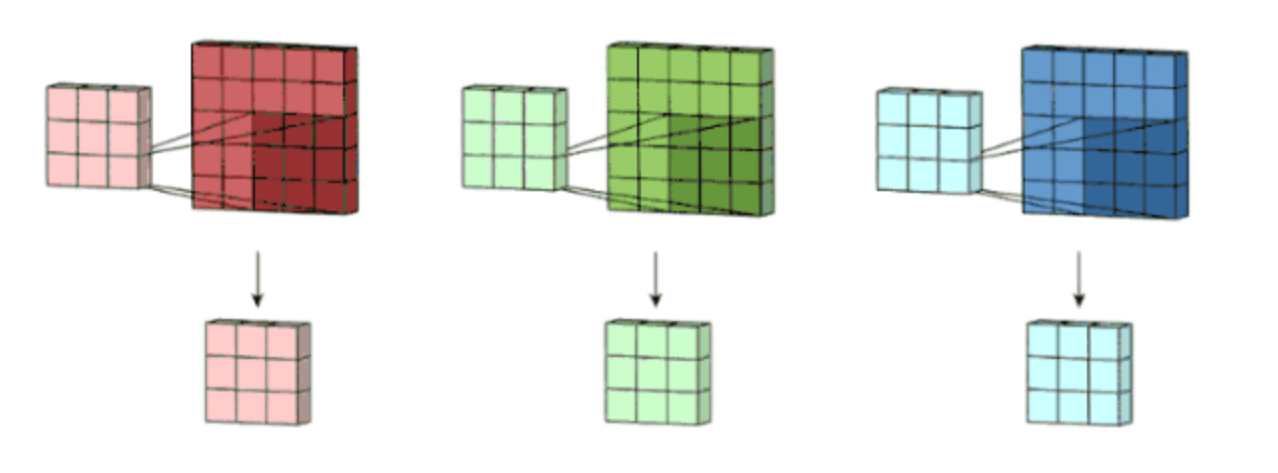
\includegraphics[width=0.5\linewidth]{./img/code/CNN/2-0}
			\end{minipage}	
		}
		
		\subfigure{
			\begin{minipage}[t]{\linewidth}
				\centering
				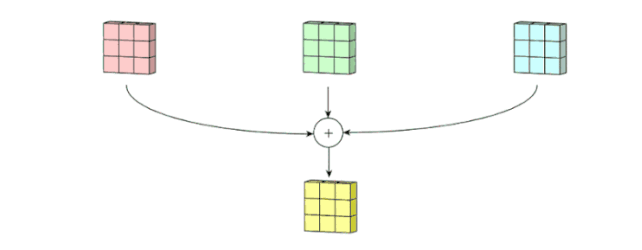
\includegraphics[width=0.5\linewidth]{./img/code/CNN/2-1}
			\end{minipage}	
		}	
		\caption{多通道卷积}
	\end{figure}
	\item 3D卷积,上面两种虽然实现了空间卷积,但是本质上还是2D卷积。而在3D卷积中,过滤器的深度要比输入层的深度要小,结果是,3D过滤器可以沿着3个方向移动。输出的数值同样也以3D空间的形式呈现,最终输出一个3D数据。如图\ref{3d_conv}.
	\begin{figure}[H]
		\centering
		\label{3d_conv}
		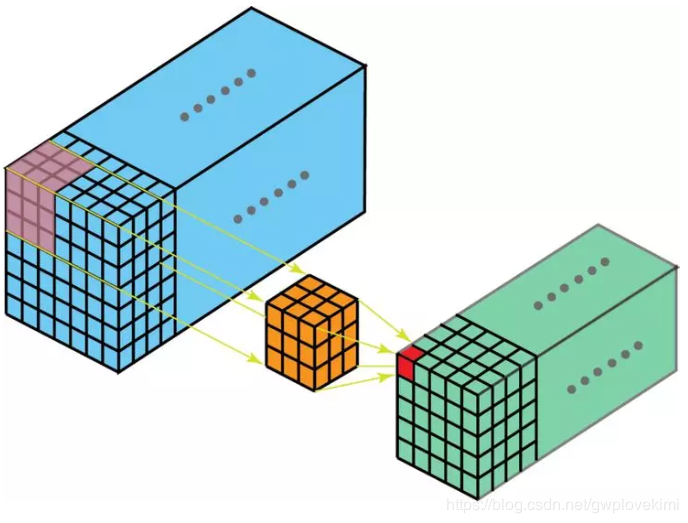
\includegraphics[width=0.3\linewidth]{./img/code/CNN/5}
		\caption{3D卷积}
	\end{figure}
	\item $1\times 1$卷积,计算上等于各个通道的加权和,同时可以改变特征通道数。如图\ref{1_conv}
	\begin{figure}[H]
		\label{1_conv}
		\centering
		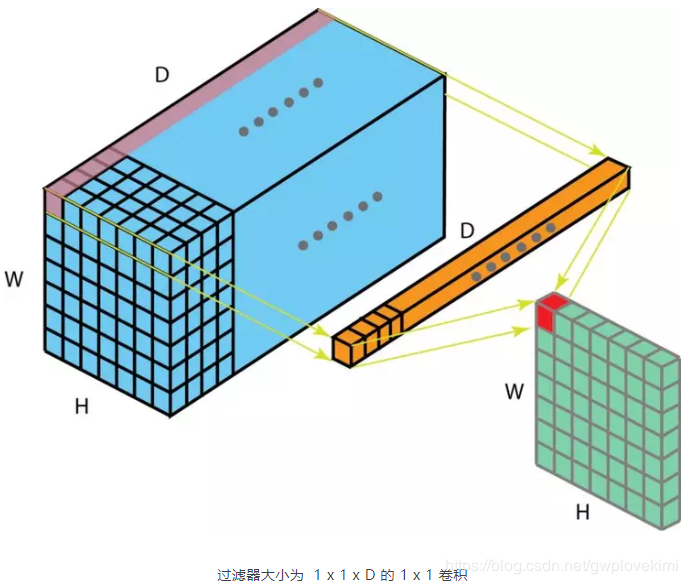
\includegraphics[width=0.3\linewidth]{./img/code/CNN/6}
		\caption{$1\times 1$卷积}
	\end{figure}
	\item 空间可分离卷积(Depthwise Separable Convolutions),我们可以将可分离卷积操作拆成多个步骤。减少计算量。如图\ref{space_sep_conv}
	\begin{figure}[H]
		\label{space_sep_conv}
		\centering
		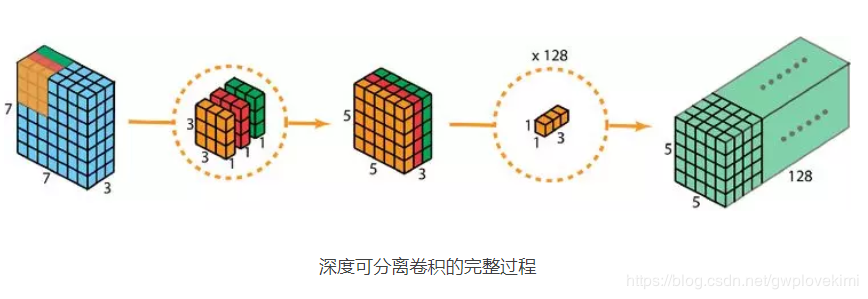
\includegraphics[width=0.5\linewidth]{./img/code/CNN/8}
		\caption{空间可分离卷积}
	\end{figure}
	\item 分组卷积(Group Convolutions),过滤器被拆分为不同中的组,每一个组负责具有一定深度的传统2D卷积的工作。另外,分组卷积也许有提供比标准完整2D卷积更好的模型。原因和稀疏过滤器有关。如图\ref{g_conv}
	\begin{figure}[H]
		\label{g_conv}
		\centering
		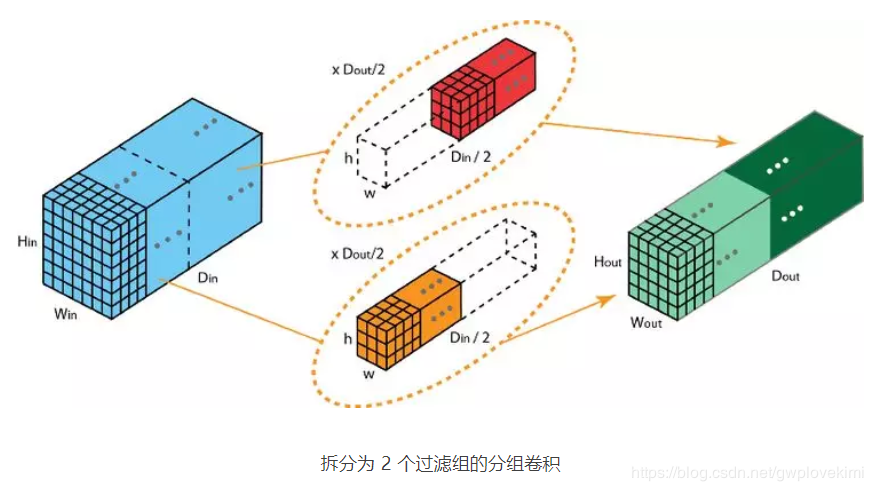
\includegraphics[width=0.5\linewidth]{./img/code/CNN/9}
		\caption{分组卷积}
	\end{figure}
	\item 扩张卷积(空洞卷积 Dilated Convolutions) ,引入另一个卷积层的参数被称为扩张率。这定义了内核中值之间的间距。扩张率为$2$的$3\times 3$的内核具有与$5\times 5$的内核相同的视野,而只使用9个参数。系统能以相同的计算成本,提供更大的感受野。如图\ref{d_conv}
	\begin{figure}[H]
		\label{d_conv}
		\centering
		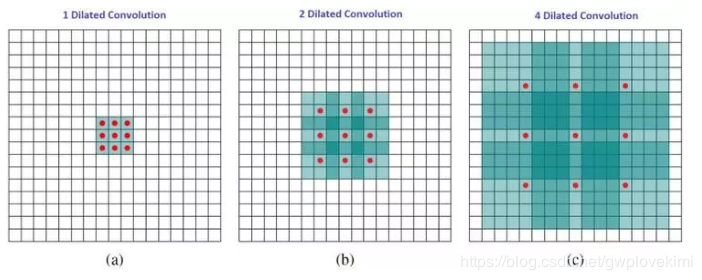
\includegraphics[width=0.5\linewidth]{./img/code/CNN/10}
		\caption{扩张卷积}
	\end{figure}
	\item 反卷积(转置卷积 Transposed Convolutions),转置卷积并非信号处理中的卷积运算的逆运算。对于 很多网络架构的很多应用言,我们往往需要进行与普通卷积方向相反的转换,即我们希望执行上采样。此时可以使用转置卷积操作。如图\ref{t_conv}
	\begin{figure}[H]
		\label{t_conv}
		\centering
		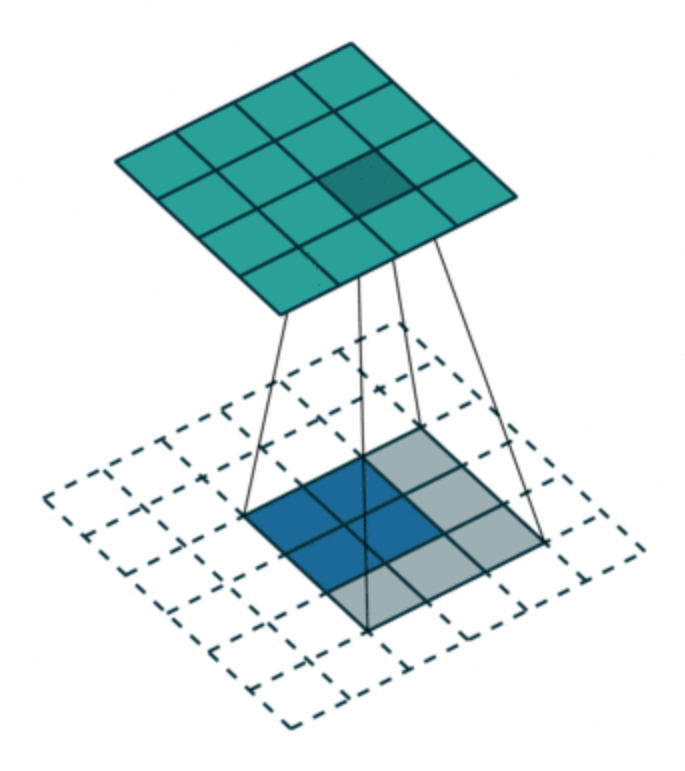
\includegraphics[width=0.3\linewidth]{./img/code/CNN/11.png}
		\caption{转置卷积}
	\end{figure}
\end{enumerate}
\subsection{卷积层的前向传播}
为简单起见,考虑单通道的情况
\begin{equation}
	\boldsymbol{X} * \boldsymbol{K} = \boldsymbol{Y}
\end{equation}
即
\begin{equation}
	\begin{pmatrix}
	x_{11}&  x_{12}& x_{13} \\ 
	x_{21}&  x_{22}&  x_{23}\\ 
	x_{31}&  x_{32}& x_{33}
	\end{pmatrix} * 
	\begin{pmatrix}
	k_{11}& k_{12} \\ 
	k_{21}& k_{22}
	\end{pmatrix} =
	\begin{pmatrix}
	y_{11}& y_{12} \\ 
	y_{21}& y_{22}
	\end{pmatrix} 
\end{equation}
这里
\begin{equation}
	\begin{aligned}
	\begin{pmatrix}
	y_{11}\\ 
	y_{12}\\ 
	y_{21}\\ 
	y_{22}
	\end{pmatrix} &= 
	\begin{pmatrix}
	x_{11}k_{11} +x_{12}k_{12} +x_{21}k_{21} +x_{22}k_{22} \\ 
	x_{12}k_{11} +x_{13}k_{12} +x_{22}k_{21} +x_{23}k_{22}\\
	x_{21}k_{11} +x_{22}k_{12} +x_{31}k_{21} +x_{32}k_{22}\\
	x_{22}k_{11} +x_{23}k_{12} +x_{32}k_{21} +x_{33}k_{22}
	\end{pmatrix}\\
	&=\begin{pmatrix}
	x_{11} &x_{12} &x_{21} &x_{22}  \\ 
	x_{12} &x_{13} &x_{22} &x_{23} \\
	x_{21} &x_{22} &x_{31} &x_{32} \\
	x_{22} &x_{23} &x_{32} &x_{33} 
	\end{pmatrix} \cdot 
	\begin{pmatrix}
	k_{11}\\ 
	k_{12}\\ 
	k_{21}\\ 
	k_{22}
	\end{pmatrix}
	\end{aligned}
\end{equation}
所以,卷积运算最终转化为矩阵运算。需要对原始的$\boldsymbol{X},\boldsymbol{K},\boldsymbol{Y}$进行变形操作,相应的记作$\boldsymbol{XC},\boldsymbol{KC},\boldsymbol{YC}$。多通道的情况只需要在维度上将操作扩展即可。
\subsection{卷积层的反向传播}
分析$\delta$误差反向传播过程可以简单的记忆为:如果神经网络$l+1$层某个结点的$\delta$误差要传到$l$层,我们就去找到前向传播时$l+1$层的这个结点和第$l$层的哪些结点有关系,权重是多少,那么反向传播时,$\delta$误差就会乘上相同的权重传播回来。

为了书写方便,记
\begin{equation}
	\begin{pmatrix}
		\delta_{11}\\ 
		\delta_{12}\\ 
		\delta_{21}\\ 
		\delta_{22}
	\end{pmatrix}=\nabla \boldsymbol{YC} = 
	\begin{pmatrix}
		\nabla y_{11}\\ 
		\nabla y_{12}\\ 
		\nabla y_{21}\\ 
		\nabla y_{22}
	\end{pmatrix}
\end{equation}
在反向传播中,$\delta$是从后面一层(一般是激活函数层或池化层)传过来的,是一个已知量,在此基础上求$\nabla \boldsymbol{K}, \nabla \boldsymbol{X}$
\begin{enumerate}
	\item 求$\nabla \boldsymbol{K}$
	\begin{equation}
		\nabla \boldsymbol{KC} = \boldsymbol{XC}^T\cdot \nabla \boldsymbol{YC}
	\end{equation}
	$\nabla \boldsymbol{KC}$ 只要reshape一下就可以得到$\nabla \boldsymbol{K}$
	\item 求$\nabla \boldsymbol{X}$
	
	根据反向传播公式,
	\begin{equation}
		\nabla \boldsymbol{XC} = \nabla \boldsymbol{YC} \cdot \boldsymbol{KC}^T
	\end{equation}
	但是,从$\nabla \boldsymbol{XC}$还原到$\nabla \boldsymbol{X}$不是一件容易的事,所以考虑新的计算方式。
	
	根据前向传播
	\begin{equation}
		\begin{pmatrix}
		y_{11}\\ 
		y_{12}\\ 
		y_{21}\\ 
		y_{22}
		\end{pmatrix} = 
		\begin{pmatrix}
		x_{11}k_{11} +x_{12}k_{12} +x_{21}k_{21} +x_{22}k_{22} \\ 
		x_{12}k_{11} +x_{13}k_{12} +x_{22}k_{21} +x_{23}k_{22}\\
		x_{21}k_{11} +x_{22}k_{12} +x_{31}k_{21} +x_{32}k_{22}\\
		x_{22}k_{11} +x_{23}k_{12} +x_{32}k_{21} +x_{33}k_{22}
		\end{pmatrix}
	\end{equation}
	可以计算每个$x_{ij}$的导数
	\begin{equation}
		\begin{aligned}
		\begin{pmatrix}
		\nabla x_{11} \\ 
		\nabla x_{12}\\ 
		\nabla x_{13}\\ 
		\nabla x_{21}\\ 
		\nabla x_{22}\\ 
		\nabla x_{23}\\ 
		\nabla x_{31}\\ 
		\nabla x_{32}\\ 
		\nabla x_{33}
		\end{pmatrix} &= \begin{pmatrix}
			k_{22}0 + k_{21}0 + K_{12}0+k_{11}\delta_{11} \\
			k_{22}0 + k_{21}0 + K_{12}\delta_{11}+k_{11}\delta_{12} \\
			k_{22}0 + k_{21}0 + K_{12}\delta_{12}+k_{11}0 \\
			k_{22}0 + k_{21}\delta_{11} + K_{12}0+k_{11}\delta_{21} \\
			k_{22}\delta_{11} + k_{21}\delta_{12} + K_{12}\delta_{21}+k_{11}\delta_{22} \\
			k_{22}\delta_{12} + k_{21}0 + K_{12}\delta_{22}+k_{11}0 \\
			k_{22}0 + k_{21}0 + K_{12}\delta_{21}+k_{11}0 \\
			k_{22}\delta_{21} + k_{21}\delta_{22} + K_{12}0+k_{11}0 \\
			k_{22}\delta_{22} + k_{21}0 + K_{12}0+k_{11}0 
		\end{pmatrix}\\
		&= \begin{pmatrix}
		0 & 0 & 0 & \delta_{11} \\ 
		0 & 0 & \delta_{11} & \delta_{12} \\ 
		0 & 0 & \delta_{12} & 0 \\ 
		0 & \delta_{11} & 0 & \delta_{21} \\ 
		\delta_{11} & \delta_{12} & \delta_{21} & \delta_{22} \\ 
		\delta_{12} & 0 & \delta_{22} & 0 \\ 
		0 & \delta_{21} & 0 & 0 \\ 
		\delta_{21} & \delta_{22} & 0 & 0 \\ 
		\delta_{22} & 0 & 0 & 0
		\end{pmatrix} \cdot 
		\begin{pmatrix}
			k_{11}\\ 
			k_{12}\\ 
			k_{21}\\ 
			k_{22}
		\end{pmatrix}
		\end{aligned}
	\end{equation}
	设上面三个矩阵分别为$\nabla \boldsymbol{X}^{'},\nabla \boldsymbol{Y}^{'},\nabla \boldsymbol{K}^{'}$,即$\nabla \boldsymbol{X}^{'}=\nabla \boldsymbol{Y}^{'}\cdot \nabla \boldsymbol{K}^{'}$。从而可见
	\begin{equation}
		\nabla \boldsymbol{X} = 
		\begin{pmatrix}
		\nabla x_{11}&\nabla  x_{12}&\nabla x_{13} \\ 
		\nabla x_{21}&\nabla  x_{22}&\nabla  x_{23}\\ 
		\nabla x_{31}&\nabla  x_{32}&\nabla x_{33}
		\end{pmatrix} = \begin{pmatrix}
		0 & 0 & 0 & 0 \\ 
		0 & \delta_{11} & \delta_{12} & 0 \\ 
		0 & \delta_{21} & \delta_{22} & 0 \\ 
		0 & 0 & 0 & 0
		\end{pmatrix} *
		\begin{pmatrix}
		k_{22} & k_{21} \\ 
		k_{12} & k_{11}
		\end{pmatrix} 
	\end{equation}
	这是一个卷积运算。不同的是对$\nabla \boldsymbol{Y}$进行卷积,从后向前卷积,有的文章称为逆向卷积。
\end{enumerate}

\subsection{池化层及池化层的反向传播}
\section{ImageNet}
\section{GoogleNet}
\section{ResNet}
\section{FCN}


\chapter{循环神经网络}
\section{RNN}
\subsection{RNN前向传播}
简单起见,我们考虑一个无偏差项的循环神经网络,且激活函数为恒等映射($\phi(x)=x$)。设时间步 $t$ 的输入为单样本 $\boldsymbol{x}_t \in \mathbb{R}^d$,标签为 $y_t$,那么隐藏状态 $\boldsymbol{h}_t \in \mathbb{R}^h$的计算表达式为

$$
\boldsymbol{h}_t = \boldsymbol{W}_{hx} \boldsymbol{x}_t + \boldsymbol{W}_{hh} \boldsymbol{h}_{t-1},
$$

其中$\boldsymbol{W}_{hx} \in \mathbb{R}^{h \times d}$和$\boldsymbol{W}_{hh} \in \mathbb{R}^{h \times h}$是隐藏层权重参数。设输出层权重参数$\boldsymbol{W}_{qh} \in \mathbb{R}^{q \times h}$,时间步$t$的输出层变量$\boldsymbol{o}_t \in \mathbb{R}^q$计算为

$$
\boldsymbol{o}_t = \boldsymbol{W}_{qh} \boldsymbol{h}_{t}.
$$

设时间步$t$的损失为$\ell(\boldsymbol{o}_t, y_t)$。时间步数为$T$的损失函数$L$定义为

$$
L = \frac{1}{T} \sum_{t=1}^T \ell (\boldsymbol{o}_t, y_t).
$$

我们将$L$称为有关给定时间步的数据样本的目标函数。
\begin{figure}[h]
	\centering
	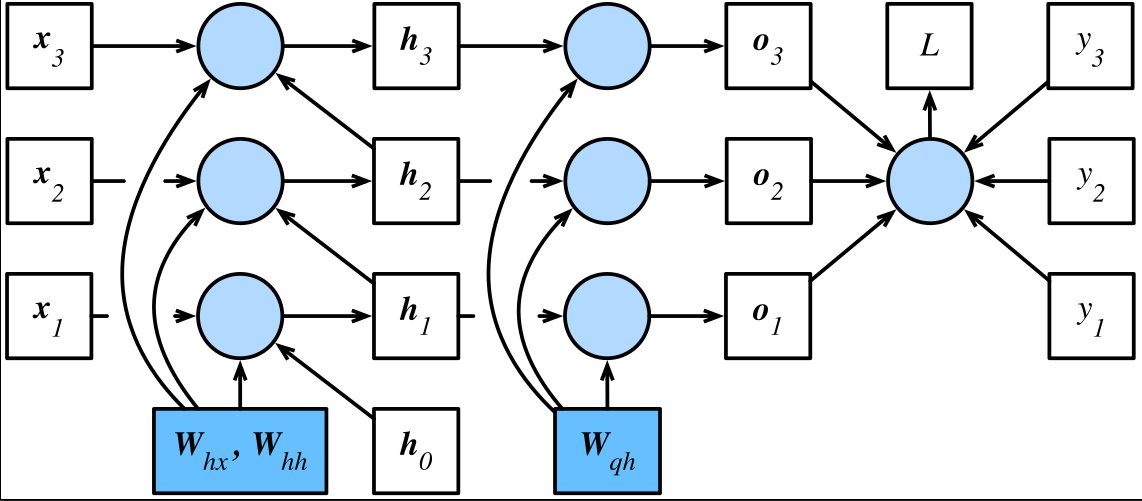
\includegraphics[width=\textwidth]{./img/code/RNN/ttbp.png}
\end{figure}

\subsection{通过时间反向传播}

模型的参数是 $\boldsymbol{W}_{hx}$, $\boldsymbol{W}_{hh}$ 和 $\boldsymbol{W}_{qh}$。链式法则的运算符用prod表示。
\begin{enumerate}
	\item $\partial L/\partial \boldsymbol{W}_{qh}$
	\begin{equation}
		\frac{\partial L}{\partial \boldsymbol{W}_{qh}} 
		= \sum_{t=1}^T \text{prod}\left(\frac{\partial L}{\partial \boldsymbol{o}_t}, \frac{\partial \boldsymbol{o}_t}{\partial \boldsymbol{W}_{qh}}\right) 
		= \sum_{t=1}^T \frac{\partial L}{\partial \boldsymbol{o}_t} \boldsymbol{h}_t^\top.
	\end{equation}
	\item $\partial L/\partial \boldsymbol{W}_{hx}$
	\begin{equation}
		\frac{\partial L}{\partial \boldsymbol{W}_{hx}} 
		= \sum_{t=1}^T \text{prod}\left(\frac{\partial L}{\partial \boldsymbol{h}_t}, \frac{\partial \boldsymbol{h}_t}{\partial \boldsymbol{W}_{hx}}\right) 
		= \sum_{t=1}^T \frac{\partial L}{\partial \boldsymbol{h}_t} \boldsymbol{x}_t^\top
	\end{equation}
	\item $\partial L/\partial \boldsymbol{W}_{hh}$
	\begin{equation}
		\frac{\partial L}{\partial \boldsymbol{W}_{hh}} 
		= \sum_{t=1}^T \text{prod}\left(\frac{\partial L}{\partial \boldsymbol{h}_t}, \frac{\partial \boldsymbol{h}_t}{\partial \boldsymbol{W}_{hh}}\right) 
		= \sum_{t=1}^T \frac{\partial L}{\partial \boldsymbol{h}_t} \boldsymbol{h}_{t-1}^\top.
	\end{equation}
\end{enumerate}
其中,目标函数有关各时间步输出层变量的梯度$\partial L/\partial \boldsymbol{o}_t \in \mathbb{R}^q$很容易计算:
\begin{equation}
	\frac{\partial L}{\partial \boldsymbol{o}_t} =  \frac{\partial \ell (\boldsymbol{o}_t, y_t)}{T \cdot \partial \boldsymbol{o}_t}.	
\end{equation}
目标函数有关时间步隐藏状态的梯度$\partial L/\partial \boldsymbol{h}_t \in \mathbb{R}^h$。依据链式法则,我们得到
\begin{equation}
	\frac{\partial L}{\partial \boldsymbol{h}_t} 
	= \sum_{i=t}^T {\left(\boldsymbol{W}_{hh}^\top\right)}^{T-i} \boldsymbol{W}_{qh}^\top \frac{\partial L}{\partial \boldsymbol{o}_{T+t-i}}.
\end{equation}
由上式中的指数项可见,当时间步数 $T$ 较大或者时间步 $t$ 较小时,目标函数有关隐藏状态的梯度较容易出现衰减和爆炸。这也会影响其他包含$\partial L / \partial \boldsymbol{h}_t$项的梯度。


\section{LSTM}
\section{GRU}
\section{Transform}
\section{Bert}

\chapter{图神经网络}
\section{GNN}
\section{GCN}
%%%%%%
\begin{appendices}
	
\end{appendices}

\end{document}

